\documentclass{article} % For LaTeX2e
\usepackage{cos424,times}
\usepackage{url}
\usepackage{graphicx}
\usepackage{hyperref}
\usepackage{multirow}
\usepackage{amsmath}
\usepackage{listings}
\usepackage{csquotes}
\usepackage{subcaption}
\usepackage{multirow}

\lstset{
    basicstyle=\small\ttfamily,
    columns=flexible,
    breaklines=true
}

\title{Predicting transactions in Bitcoin blockchain data}

\author{
Gregory Gundersen\\
Princeton University\\
\texttt{ggundersen@princeton.edu}
\And
Prakhar Kumar \\
Princeton University \\
\texttt{prakhark@princeton.edu} \\
}

\newcommand{\fix}{\marginpar{FIX}}
\newcommand{\new}{\marginpar{NEW}}

\begin{document}

\maketitle

\begin{abstract}
We predict future Bitcoin transactions for pairs of addresses based on historical transaction data. The training dataset consists of transaction counts between sender-receiver address pairs that interacted within a one-year period. The test data consists of address pairs which did not interact within that one year period but may have in the future. We convert the training dataset into an extremely sparse adjacency matrix of all possible combinations of addresses with each entry corresponding to the number of transactions and then use matrix completion methods to reconstruct a low-rank approximation of the data which can be used for prediction. We find that two matrix completion methods, singular value decomposition and nonnegative matrix factorization, generalize significantly better than random guessing.
\end{abstract}

\section{Introduction}

\subsection{Background}

Bitcoin is an online virtual currency introduced in 2008 by Satoshi Nakamoto \cite{nakamoto2008bitcoin}. All transactions are cryptographically signed and recorded on a public ledger called the blockchain. The blockchain allows the global, peer-to-peer network of Bitcoin users to validate all transactions and thereby eschew a centralized bank. See \cite{nielsen2013bitcoin} for a detailed explanation of how Bitcoin works. The upshot is that with Bitcoin, everyone is the bank and the blockchain is an account of the entire history of all anonymized transactions.

In this paper, we predict transactions between pairs of addresses in a portion of the Bitcoin blockchain. The training dataset consists of transaction counts between sender-receiver address pairs that did interact, i.e. there are no zero counts, within a one year period. Therefore the entire training dataset consists of positive examples. The testing dataset consists of some pairs of addresses which did not interact and some which did in a subsequent year. We find that matrix completion methods to estimate the probability of transactions between a sender-receiver pair work better than traditional classification models. In particular, we investigate two matrix completion methods, singular value decomposition (SVD) and nonnegative matrix factorization (NMF). Their performances were evaluated on accuracy, precision, recall, and area under the curve (AUC). We found that NMF generalizes better on the test data in comparison to SVD.

In addition, we explored an SVM-based classifier on a modified dataset in which the additional features are the indegree and outdegree of both the receiver and sender. However, we found that the test accuracy was always around 90\% with low accuracy and recall despite constructing a balanced training set consisting of equal number of positive and negative labels.

\subsection{Related work}

Matrix completion methods are frequently used for recommender systems \cite{koren2009matrix}. This is because recommender systems typically rely on incomplete and/or sparse data to provide suitable recommendations to the users for services like Amazon, Facebook, and Netflix. The sparsity is common because in most scenarios a user cannot rate or even be aware of most items. The central challenge, then, is to develop methods to fill in missing recommendations based on the user and others' recommendations. The key assumption is that user preferences are generally guided by a small number of underlying factors and so decomposing the data into a low-rank representation creates a more general model.

This approach can be used for this work predicting Bitcoin transactions because we assume the number of factors which determine whether or not two users will interact is much smaller than the number of addresses in the dataset. The significant sparsity of our dataset makes it ideal to implement matrix factorization methods for identifying low-rank decompositions of the original data.

The Netflix Prize is a popular example of recommender systems employing large scale SVD and other matrix completion methods to estimate the probable preferences of users for movies \cite{bennett2007netflix}.

\section{Methods}

\subsection{Data}

\paragraph{Description.} The training dataset consists of transactions between 3,348,026 sender-receiver pairs and the number of times the sender paid the receiver. The transactions were made between March 2012 to March 2013. The testing dataset consists of sender-receiver pairs which did not interact in the training set time period but may have by the following year, May 2014. The full dataset contains 444,075 unique addresses, and therefore over 19.7 billion possible unordered pairs of addresses. A binary adjacency matrix is extremely sparse, with only $1.7 \times 10^{-5}$ nonzero values.

\paragraph{Exploration.} To better understand the data, we constructed a smaller dataset with three columns: address, outdegree, and indegree. We found a positive correlation between indegree and outdegree (Figure \ref{fig:degree_address}). Surprisingly, while some nodes have high outdegree without a high indegree, no nodes have a high indegree but a low outdegree. We expected the opposite: online merchants would receive many payments but not send money often.

In addition, we also found a strong relationship between the address and the outdegree (Figure \ref{fig:in_out_degree}) and indegree (not shown). Lower address numbers have higher indegrees and outdegrees. This suggests that the addresses themselves will be useful as features.

\begin{figure}
\centering
\begin{subfigure}{.5\textwidth}
    \centering
    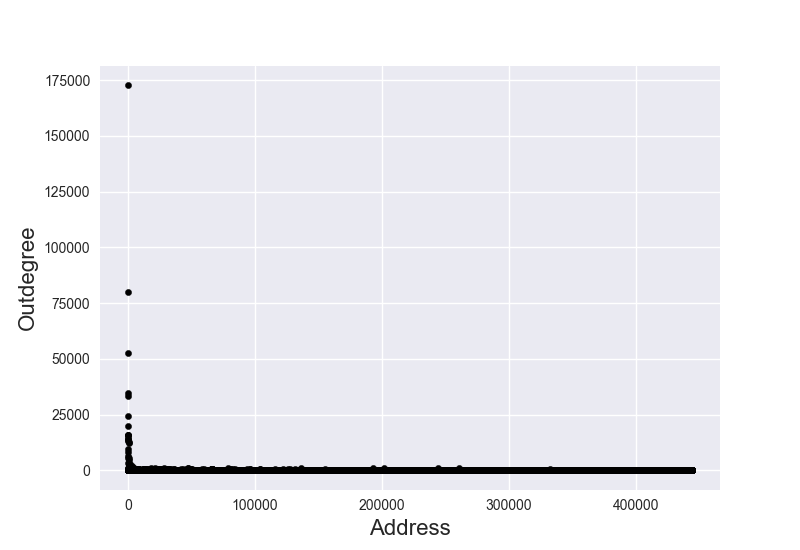
\includegraphics[width=1\linewidth]{figures/degree_address}
    \caption{\small TK TK}
    \label{fig:degree_address}
\end{subfigure}%
\begin{subfigure}{.5\textwidth}
    \centering
    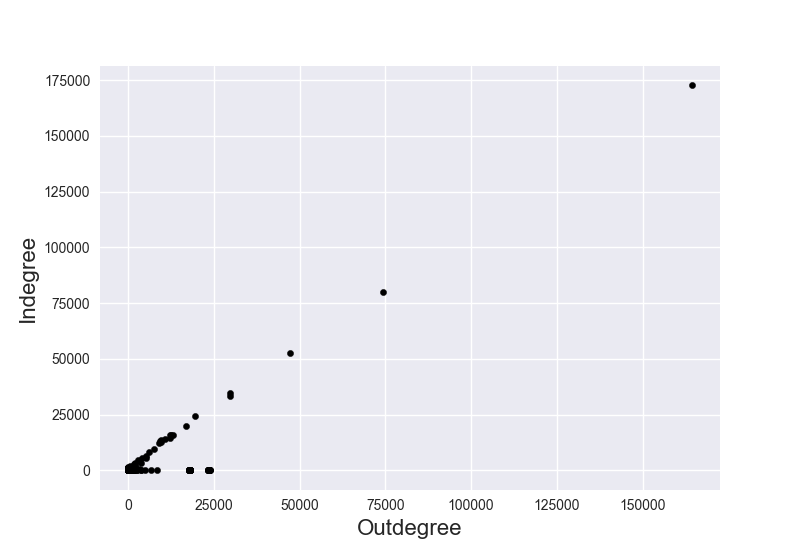
\includegraphics[width=1\linewidth]{figures/in_out_degree}
    \caption{\small TK TK}
    \label{fig:in_out_degree}
\end{subfigure}
\caption{\small TK TK}
\label{fig:test}
\end{figure}

\subsection{Feature selection}

We approached prediction through two views of the data: matrix completion of a binary adjacency matrix and supervised learning on a dataset with graph properties as features.

For matrix completion, the dataset is a $444,075 \times 444,075$ adjacency matrix, far too large to store in memory. We used the Python library \texttt{scipy} for several representations of sparse matrices which work with \texttt{scikit-learn}'s SVD, NMF, and LDA implementations \cite{jones2014scipy} \cite{scikit-learn}.

For supervised learning, we generated a new dataset with six features of the implicit graph in the transaction dataset: (1) sender address, (2) receiver address, (3), sender outdegree, (4) sender indegree, (5) receiver outdegree, and (6) receiver indegree. The number of transactions was dropped from the training dataset because it is not available in the test dataset. We tested two supervised classifiers on this dataset, SVM and logistic regression. Because a full dataset of all possible combinations of addresses is too large (over 19.7 billion samples), we subsampled the dataset, selecting 1,000,000 samples with a hyperparameter $pp$ indicating the percent positive.

\subsection{Classifiers}\label{classifiers}

\paragraph{Spotlight: Nonnegative matrix factorization}\label{Spotlight}

Nonnegative matrix factorization (NMF) is a method for approximating a matrix as the outer product of two other, typically smaller, matrices. Formally, a matrix $X$ is factorized into matrices $V$ and $U$ such that:

\begin{equation} \label{eq:1}
X \approx V \times U
\end{equation}

Where $X$ is an $n \times m$ matrix, $V$ is an $n \times k$ matrix, and $U$ is a $k \times m$ matrix. The value $k$ is a hyperparameter of the model which indicate the number of latent variables that approximate $V$ (Figure \ref{fig:matrix_completion}).

\begin{figure}[!htbp]
    \centering
    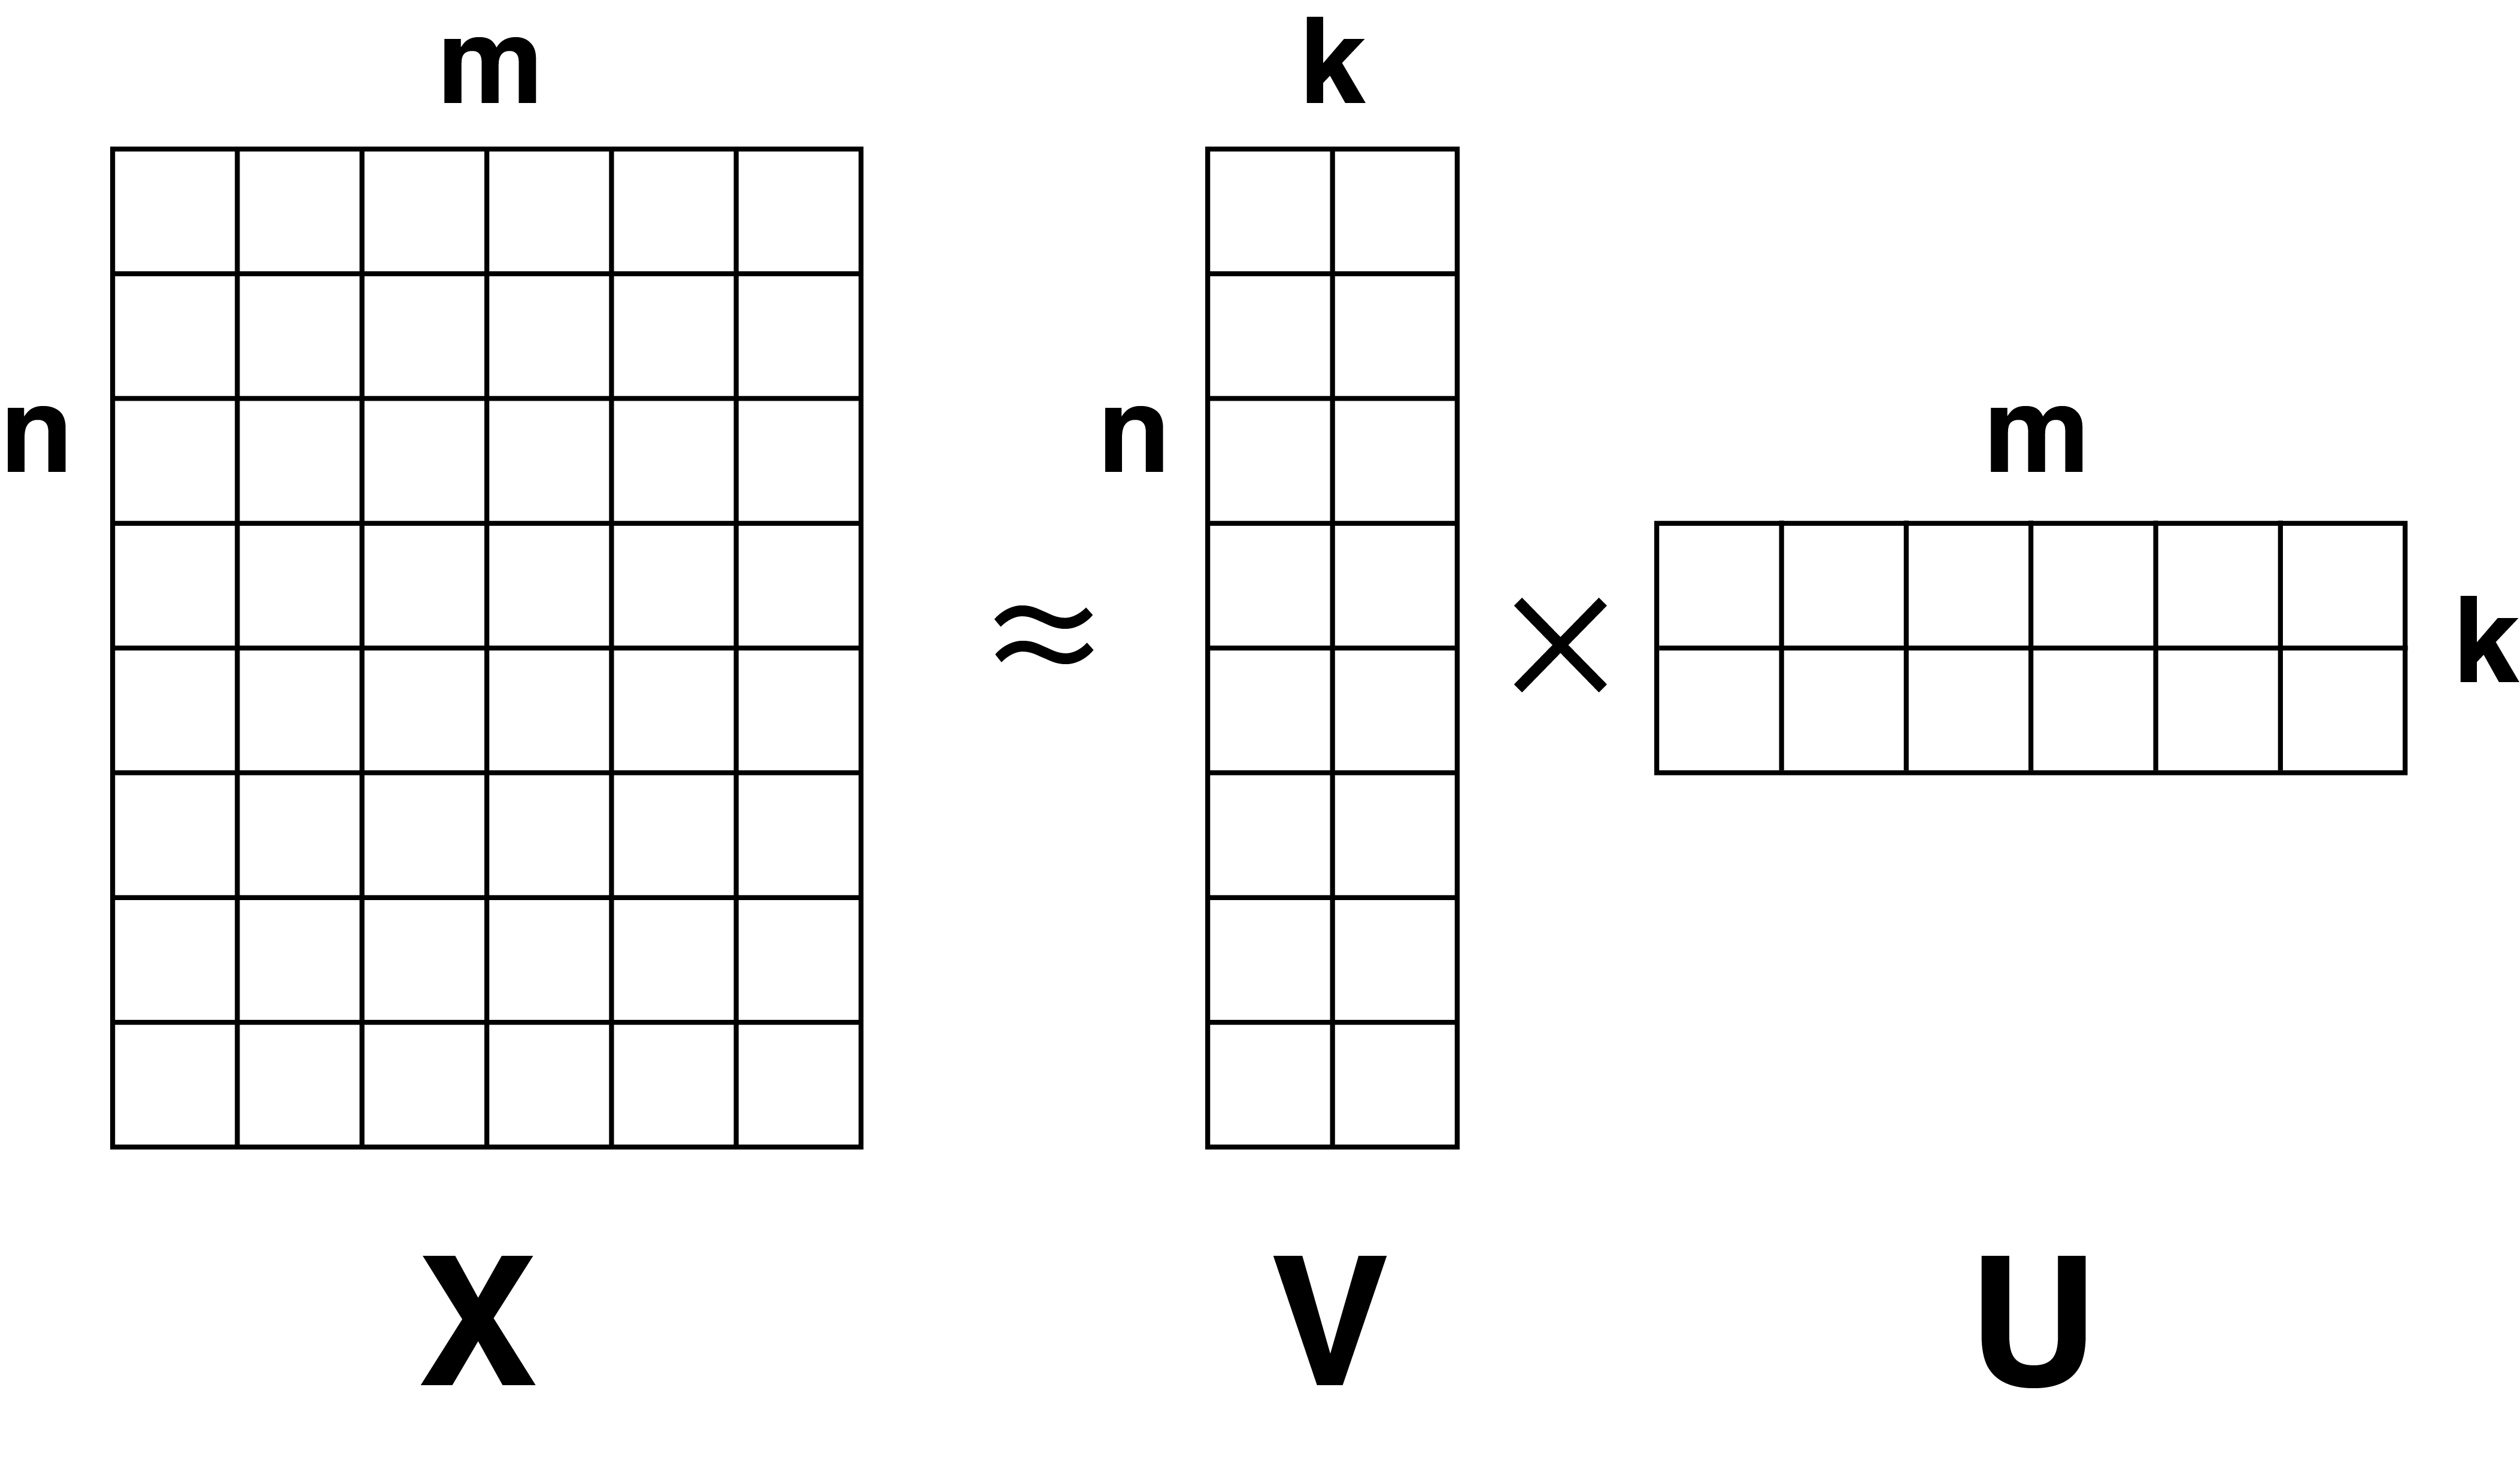
\includegraphics[scale=0.2]{figures/matrix_completion}
    \caption{\small Matrix $X$ is factorized into matrices $V$ and $U$.}
    \label{fig:matrix_completion}
\end{figure}

The key assumption is that the approximated matrix has low-rank. In other words, not every cell in the matrix is a free variable. Instead, each cell value is the dot product of two $k$-dimensional vectors. The value of the low-rank assumption is that it reduces the number of free parameters of a model. In the most extreme case, $k=1$, a model that would typically have $n \times m$ parameters can be approximated by just $n + m$ parameters. In general, the number of parameters is $k \times (n + m)$.

Prediction for matrix completion methods such as NMF are as follows. First, we approximate the observed data $X$ using matrix factorization (Equation \ref{eq:1}). We then complete the matrix by multiplying the two matrix factors together:

$$
\hat{X} = V \times U
$$

In principle, $\hat{X}$ is a matrix that captures the latent structure in $X$. We can then base predictions on the value in the completed matrix. For example, since our matrix $X$ contains sender addresses as rows and receiver addresses as columns (or vice versa), then the prediction for whether or not the $i$th address made a transaction with the $j$th address would be found in $\hat{X}[i, j]$.

There are many algorithms for solving matrix factorization for NMF. See \cite{lee2001algorithms} for details. One straightforward way is to use gradient descent to minimize the difference between the observed data and the factorized estimates. Formally, given observation $X_{ij}$, we want to find low-dimensional vectors $v$ and $u$ such that $X_{ij} = v_i \cdot  u_j$ by minimizing the following objective function:

$$
f(u, v) = \sum_{i,j \text{ observed}} (X_{ij} - v_i \cdot u_j)^2
$$

Ultimately, the learned matrices $V$ and $U$ are uninterpretable. But like many machine learning methods, we assume that if we can approximate the data well with fewer numbers, we might capture generalities in the data. Other dimensionality reduction methods such as SVD and PCA rely on this thinking as well.

\paragraph{Classifiers.} We used four classifiers from the \texttt{scikit-learn} Python library \cite{scikit-learn}, two which make predictions on graph features and two which use matrix completion. Unless stated otherwise, we used the default parameters for each classifier as implemented by \texttt{scikit-learn}.

\emph{Supervised learning classifiers.}

\begin{itemize}

\item \textbf{Support Vector Machine} (SVM): Linear classification with hinge loss. \texttt{scikit-learn}'s default \texttt{SVC} class was extremely slow, so we trained a \texttt{SGDClassifier} with hinge loss online for 100 batches with a batch size of 100000 and 0.1\% positive examples.

\item \textbf{Logistic Regression} (LR): Regression with binary classification. We trained the model on a subsample of the full dataset ($n = 1,000,000$) with varying percentages of positive examples ($pp$).

\end{itemize}

\emph{Matrix completion classifiers.}

\begin{itemize}

\item \textbf{Singular Value Decomposition.} (SVD): is a matrix factorization and dimensionality reduction technique.

\item \textbf{Nonnegative Matrix Factorization} (NMF): Factorizes the observed data matrix $X$ into two lower-dimensional matrices. A new matrix $\hat{X}$ can be reconstructed and used for prediction. See Section \ref{Spotlight} for details.

Non-negative matrix factorization is another well-known matrix completion technique. It is especially useful for decomposition of multivariate data into product of two non-negative matrices. By restricting the rank of the matrices we can create a dense low rank approximation of the data and extract the underlying meaningful structures in the data.

\item \textbf{Latent Dirichlet Allocation} (LDA): Statistical model that explains why latent groups in the data are similar. We used $\text{\detokenize{n_topics}}=5$.

\end{itemize}

\section{Results}

The results for the performance of SVD and NMF were evaluated on various metrics such as accuracy score, precision, recall and F-1 score. The results have been summarized in Table [TK table]. Moreover, ROC curves for both the methods were analyzed to compare the performances for varying classification thresholds [TK table] . It can be clearly observed from the two ROC curves that NMF outperforms the SVD since the performance of SVD based approach falls below the random guess at a certain threshold.

\begin{table}
\centering
{
\fontsize{10}{14}\selectfont
\noindent\begin{tabular}{ c | c | c c c | c c c c | c | c }
	\hline
	    & \multirow{2}{*}{SVM}
	    & \multicolumn{3}{c|}{LR}
	    & \multicolumn{4}{c|}{NMF}
	    & \multirow{2}{*}{LDA}
	    & \multirow{2}{*}{SVD} \\
	\cline{3-9}
    & & pp=0.5 & pp=0.1 & pp=0.01 & k=5 & k=10 & k=20 & k=50 & & \\
	\hline
	\hline
	Accuracy  & 0.8430 & 0.6235 & 0.8580 & 0.8942 & 0.8891 & 0.8696 & 0.8449 & 0.8468 & 0.1000 & 0.8380 \\
	\hline
	Precision & 0.3339 & 0.1755 & 0.3697 & 0.4744 & 0.4350 & 0.3584 & 0.2880 & 0.2940 & 0.1000 & 0.2629 \\
	\hline
	Recall    & 0.5730 & 0.7480 & 0.5960 & 0.5370 & 0.3680 & 0.3850 & 0.3760 & 0.3800 & 0.5868 & 0.6380 \\
	\hline
	F1 score  & 0.4219 & 0.2844 & 0.4564 & 0.5038 & 0.3989 & 0.3712 & 0.3265 & 0.3315 & 1.0000 & 0.3440 \\
	\hline
	AUC       & 0.7230 & 0.6788 & 0.7416 & 0.7354 & 0.7320 & 0.7329 & 0.7230 & 0.7337 & 0.1818 & 0.2980 \\
	\hline
\end{tabular}
}
\caption{\small TK TK}
\label{tab:standardresults}
\end{table}

\paragraph{SVM and Logistic regression.} TK TK.

\paragraph{NMF.} TK TK.

\begin{figure}
\centering
\begin{subfigure}{.5\textwidth}
    \centering
    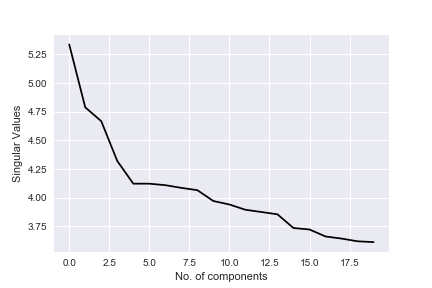
\includegraphics[width=1\linewidth]{figures/singular_values_log_yscale}
    \caption{\small TK TK}
    \label{fig:svd}
\end{subfigure}%
\begin{subfigure}{.5\textwidth}
    \centering
    \includegraphics[width=1\linewidth]{figures/roc}
    \caption{\small TK TK}
    \label{fig:roc}
\end{subfigure}
\caption{\small TK TK}
\label{fig:test}
\end{figure}

\paragraph{SVD.} In order to decompose the large sparse data matrix as a product of two low-rank matrices, we analyzed the singular values by plotting these singular values for different components. We decided to select the top 20 components by observing a ``knee'' in the plot (Figure \ref{fig:svd}). Thus, the assumption was that the basic factors determining whether a transaction would take place can be explained by these 20 components.

\section{Discussion}

This work has attempted at identifying the possibility of future transactions between previously unrelated addresses. Matrix completion methods have been used as the tools for doing the same.

\subsubsection*{Acknowledgments}

We benefited from class notes, precept discussion, and office hours for Princeton's COS 424.

\bibliography{ref}
\bibliographystyle{plain}

\end{document}
